\documentclass{beamer}

\usepackage{graphicx}
\usepackage{hyperref}
\usepackage[latin1]{inputenc}
\usepackage[T1]{fontenc}
\usepackage[english]{babel}
\usepackage{listings}
\usepackage{xcolor,mathrsfs,url}
\usepackage{amssymb}
\usepackage{amsmath}
\usepackage{ifthen}
\usepackage{tikz}
\usepackage{tikz-qtree}
\usepackage{eurosym}
\everymath{\displaystyle}

% The command to define a subsection is '\subsec{}' and NOT '\subsection'.
% This code generates the bar. Don't edit.
\newcommand{\midbarnew}{}
\newcommand{\subsec}[1]
{
  \ifthenelse{\equal{#1}{}}
  {\renewcommand{\midbarnew}{} \subsection{}}
  {\renewcommand{\midbarnew}{ $\mid$ } \subsection{#1}}
}

% change the pictures here, if necessary. logobig and logosmall are the internal names
% for the pictures: do not modify them, just change "hulogo" and "logo". Pictures must be 
% supplied as JPEG, PNG or PDF
%########################################

\pgfdeclareimage[height=2cm]{logobig}{logo} % use hucase instead for the Humboldt-Case Logo
\pgfdeclareimage[height=1cm]{logosmall}{logo}

% use this number to modify the scaling of the headline on titlepage
\def\titlescale{1.0}


\title{Purchasing Power Parity}
\author{Instructor: David Jinkins\thanks{I wish to acknowledge Battista Severgnini for providing last year's slides to me. His generosity saved me much time, and these slides are partially based on his. Any errors are of course my own.}}
\date{Date: Oct. 6, 2014}
%Start of the document
\begin{document}

\frame[plain]{% create the titleslide, layout controlled in metricsbeamer
	\titlepage
}

\frame{% how to print
\frametitle{Last Time}
\begin{itemize}
    \item Chapter 15
    \begin{itemize}
    \item Money
    \begin{itemize}
        \item What is special about it?
        \item How is it measured?
        \item What determines how much people want?
    \end{itemize}
    \item A Short-run model of the money market
    \item Adjustment in the Long-run
    \begin{itemize}
        \item Why exchange rates are so volatile
    \end{itemize}
    \end{itemize}
    \item Chapter 16
    \begin{itemize}
        \item The law of one price
        \item Purchasing Power Parity
        \item Relative vs. Absolute PPP
    \end{itemize}
    \end{itemize}
}

\frame[plain]{
\frametitle{This time}
\begin{itemize}
    \item Chapter 16:
    \begin{itemize}
        \item Purchasing Power Parity
        \begin{itemize}
            \item The law of one price
            \item Relative vs. Absolute PPP
        \end{itemize}
        \item Exchange rates and PPP
        \begin{itemize}
            \item Long-run, monetary approach
            \item Clash of predictions
            \item Fisher effect
        \end{itemize}
        \item Empirical evidence on PPP
        \begin{itemize}
            \item It bad
            \item Why it bad
        \end{itemize}
        \item A generalized PPP model
        \begin{itemize}
            \item Real exchange rate
            \item Interest and the real exchange rate 
            \item Real interest rate parity
        \end{itemize}
    \end{itemize}
\end{itemize}}

\begin{frame}{But first a review}
\end{frame}

% \frame[plain]{\includegraphics[page=7,width=\textwidth]{national_accounts.pdf}}
% \frame[plain]{\includegraphics[page=8,width=\textwidth]{national_accounts.pdf}}
% \frame[plain]{\includegraphics[page=9,width=\textwidth]{national_accounts.pdf}}
% \frame[plain]{\includegraphics[page=10,width=\textwidth]{national_accounts.pdf}}
% \frame[plain]{\includegraphics[page=11,width=\textwidth]{national_accounts.pdf}}
% \frame[plain]{\includegraphics[page=13,width=\textwidth]{national_accounts.pdf}}
% \frame[plain]{\includegraphics[page=28,width=\textwidth]{national_accounts.pdf}}
% \frame[plain]{\includegraphics[page=29,width=\textwidth]{national_accounts.pdf}}
% \frame[plain]{\includegraphics[page=30,width=\textwidth]{national_accounts.pdf}}
% \frame[plain]{\includegraphics[page=32,width=\textwidth]{national_accounts.pdf}}
% \frame[plain]{\includegraphics[page=40,width=\textwidth]{national_accounts.pdf}}
% \frame[plain]{\includegraphics[page=41,width=\textwidth]{national_accounts.pdf}}
% \frame[plain]{\includegraphics[page=47,width=\textwidth]{national_accounts.pdf}}
% \frame[plain]{\includegraphics[page=48,width=\textwidth]{national_accounts.pdf}}
% \frame[plain]{\includegraphics[page=53,width=\textwidth]{national_accounts.pdf}}
% \frame[plain]{\includegraphics[page=57,width=\textwidth]{national_accounts.pdf}}
% \frame[plain]{\includegraphics[page=58,width=\textwidth]{national_accounts.pdf}}
% \frame[plain]{\includegraphics[page=59,width=\textwidth]{national_accounts.pdf}}
% \frame[plain]{\includegraphics[page=60,width=\textwidth]{national_accounts.pdf}}
% \frame[plain]{\includegraphics[page=61,width=\textwidth]{national_accounts.pdf}}
% \frame[plain]{\includegraphics[page=65,width=\textwidth]{national_accounts.pdf}}
% \frame[plain]{\includegraphics[page=67,width=\textwidth]{national_accounts.pdf}}
% \frame[plain]{\includegraphics[page=71,width=\textwidth]{national_accounts.pdf}}
% \frame[plain]{\includegraphics[page=72,width=\textwidth]{national_accounts.pdf}}
% \frame[plain]{\includegraphics[page=73,width=\textwidth]{national_accounts.pdf}}
% \frame[plain]{\includegraphics[page=74,width=\textwidth]{national_accounts.pdf}}
% 
% \begin{frame}{Review}
%     \begin{itemize}
%         \item End review
%     \end{itemize}
% \end{frame}


\frame{% how to print
\frametitle{}
\begin{center}
\textcolor{blue}{Chapter 16: Price Levels and the Exchange Rate in the Long Run
}
\end{center}
}


\begin{frame}{This chapter: More long run models}

\begin{itemize}
    \item In Chapter 15, we saw short run and long run models of money supply and exchange rate
    \begin{itemize}
        \item One-time change in money supply
        \item No long run change in real money supply
        \item No long run change in interest rate
    \end{itemize}
    \item In this chapter, permanent changes in the interest rate and exchange rates
    \begin{itemize}
        \item Only possible if the growth rate of the money supply changes 
        \item Different instrument, no change in current money supply
        \item Long-run: increase in growth rate leads to depreciation of currency
        \item Model based on something called Purchasing Power Parity
    \end{itemize}
\end{itemize}

\end{frame}

\begin{frame}{How we are going to get there}

    \begin{enumerate}
        \item What is PPP?
        \item Model based on PPP
    \end{enumerate}

\end{frame}

\frame{
\frametitle{The Law of One Price}
The prices of identical goods sold in different
countries must be the same when expressed
in terms of the same currency.
\begin{itemize}
    \item The same doner kebab has to be the same price anywhere on Jagtsvej in N�rrebro
    \begin{itemize}
        \item Otherwise hipsters would mostly go to the cheapest kebab shop
        \item CBS students would buy kebab from the cheap shop, and sell outside the expensive shop for a profit 
    \end{itemize}
    \item Technically only works if customers have time and don't mind walking 
\end{itemize}
}

\frame{\frametitle{Beer}
\begin{itemize}
    \item Price of a Carlsberg can't be too different on opposite sides of the Danish-German border
    \item If we ignore transport and other border costs, \emph{law of one price}:
\begin{center}
    $P^{\mbox{beer}}_{DK} = \left(E_{DKK/EURO}\right) x \left(P^{\mbox{beer}}_{E}\right)$
\end{center}
\item where:
\begin{itemize}
\item $P^{\mbox{beer}}_{DK}$ is the DKK price of a Carlsberg when sold in DK
\item $P^{\mbox{beer}}_{E}$ is the corresponding Euro price in the Euro zone 
\item $\left(E_{USD/EURO}\right)$ is the DKK/Euro exchange rate
\end{itemize}
\end{itemize}}


\frame{
\frametitle{Purchasing Power Parity}
\begin{itemize}
    \item PPP is the application of the law of one price across countries:
        \begin{itemize}
            \item Price of a basket goods should be independent of currency 
            \item Compares general price level across countries
            \item Neither implies nor requires law of one price to hold
        \end{itemize}
    \item PPP predicts a DKK/Euro exchange rate of

\begin{center}
$ E_{DKK/EURO} =\frac{P_{DK}}{P_{E}}$
\end{center}
\item where
\begin{itemize}
\item $P_{DK}$ is the DKK price of a reference commodity basket sold in Denmark
\item $P_{E}$ is the euro price of the same basket in the Euro zone
\end{itemize}
\end{itemize}
}

\frame{
\frametitle{Purchasing Power Parity (PPP)}
\begin{itemize}
    \item PPP predicts a DKK/Euro exchange rate of
\begin{center}
$ E_{DKK/EURO} =\frac{P_{DK}}{P_{E}}$
\end{center}
    \item Rearranging,
    \begin{center}
    $ P_{DK}=\left(E_{DKK/EURO}\right)x\left(P_{E}\right)$
    \end{center}
    \item People have the same purchasing power with their currency regardless of country
    \item Prices twice as high only if currency half as valuable
\end{itemize}
}

\frame{
\frametitle{PPP \& Law of One Price}
\begin{itemize}
    \item The law of one price applies to individual commodities
    \item PPP applies to the general price level
    \item PPP neither implies nor requires law of one price
    \item But, law of one price both implies and requires PPP to hold
    \begin{itemize}
        \item If the law of one price holds true for every
commodity $\Rightarrow$ PPP must hold for the same
reference baskets across countries
        \item If PPP holds, this does not mean that law of one price is respected
    \end{itemize}
\end{itemize}
}


\frame{
\frametitle{Flavors of Purchasing Power Parity}
\begin{enumerate}
\item Absolute PPP: exchange rates equal relative price levels
\begin{center}
$ E_{DKK/EURO} =\frac{P_{DK}}{P_{E}}$
\end{center}
\item Relative PPP: the percentage change in the exchange
rate between two currencies equals the difference
between the percentage changes in national price
levels.
\begin{center}
$\frac{\left(E_{DKK/EURO,t} - E_{DKK/EURO,t-1}\right)}{ E_{DKK/EURO,t-1}}= \pi_{DK, t} - \pi_{E, t}$
\end{center}
\end{enumerate}
where $\pi_{t}$ = inflation rate from period $t-1$ to $t$
\begin{equation*}
    \pi_{t} = \frac{P_t - P_{t-1}}{P_{t-1}}
\end{equation*}
\begin{itemize}
    \item Relative PPP is an approximation of the following relation:
        \begin{equation*}
            \frac{E_{DKK/EURO,t}}{E_{DKK/EURO,t-1}} =\frac{\frac{P_{DK,t}}{P_{E,t}}}{\frac{P_{DK,t-1}}{P_{E,t-1}}}
        \end{equation*}
\end{itemize}

}


\frame{
\frametitle{Absolute \& Relative PPP}
\begin{itemize}
    \item Relative PPP is an approximation of the following relation:
        \begin{equation*}
            \frac{E_{DKK/EURO,t}}{E_{DKK/EURO,t-1}} =\frac{\frac{P_{DK,t}}{P_{E,t}}}{\frac{P_{DK,t-1}}{P_{E,t-1}}}
        \end{equation*}
    \item If absolute PPP holds $\Rightarrow$ relative PPP holds
\end{itemize}
}


\frame{
\frametitle{Absolute \& Relative PPP}
\textbf{Not the other way around!}
\begin{itemize}
    \item Relative PPP is an approximation of the following relation:
        \begin{equation*}
            \frac{E_{DKK/EURO,t}}{E_{DKK/EURO,t-1}} =\frac{\frac{P_{DK,t}}{P_{E,t}}}{\frac{P_{DK,t-1}}{P_{E,t-1}}}
        \end{equation*}
    \item Relative PPP does not imply absolute PPP 
        \begin{equation*}
            \frac{8}{4} = \frac{4}{2} \not\rightarrow 8 = 4
        \end{equation*}
\end{itemize}
}

\begin{frame}{Pause}

    \begin{itemize}
        \item We have defined the law of one price
        \item We have defined absolute PPP
        \begin{itemize}
            \item Law of one price $\rightarrow$ absolute PPP
            \item Absolute PPP $\not\rightarrow$ law of one price
        \end{itemize}
        \item We have defined relative PPP
        \begin{itemize}
            \item Absolute PPP $\rightarrow$ relative PPP
            \item Relative PPP $\not\rightarrow$ absolute PPP
        \end{itemize}
        \item Does law of one price imply relative PPP?
        \begin{itemize}
            \item Each condition weaker than the last
        \end{itemize}
        \item Next: how do changes in inflation affect exchange rate? 
    \end{itemize}

\end{frame}

\frame{
\frametitle{Long-Run Model with absolute PPP}
\begin{itemize}
    \item \emph{Monetary approach} to the exchange rate 
    \item Switch to USD and Euro to use plots from text
    \item Money demand and supply as previous:
\end{itemize}
\begin{enumerate}
\item In the United States:
\begin{center}
$P_{US}= \frac{M^{s}_{US}}{L \left(R_{USD}, Y_{US}\right)}$
\end{center}
\item In Europe:
\begin{center}
$P_{E}= \frac{M^{s}_{E}}{L \left(R_{EURO}, Y_{E}\right)}$
\end{center}
\end{enumerate}}


\frame{
\frametitle{PPP and Money Market}
\begin{center}
$E_{USD/EURO}=\frac{P_{US}}{P_{E}}=\frac{\frac{M^{s}_{US}}{L \left(R_{USD}, Y_{US}\right)}}{\frac{M^{s}_{E}}{L \left(R_{EURO}, Y_{E}\right)}}$
\end{center}
Specific Predictions:
\begin{enumerate}
\item Money supplies: if $M^{s}_{US}  \Uparrow \Rightarrow$ long-run depreciation of the dollar against the euro
\item interest rates: if $R_{USD}  \Uparrow \Rightarrow$  
causes a depreciation of the dollar against the
euro
\item Output levels: a rise if $Y_{US} \Uparrow \Rightarrow$ causes an appreciation
of the dollar against the euro.
\end{enumerate}
}

\frame{
\frametitle{Whoops!}
\begin{itemize}
    \item interest rates: if $R_{USD}  \Uparrow \Rightarrow$ causes a depreciation of the dollar against the euro
\end{itemize}
\begin{figure}
	\centering
		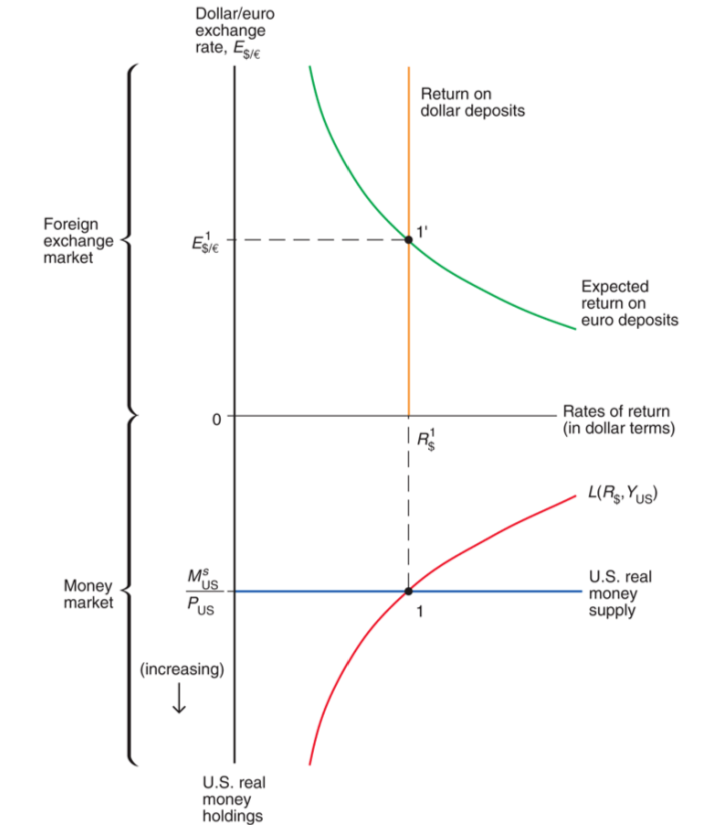
\includegraphics[scale=0.23]{money_exchange.png}
\end{figure}
}

\frame{
\frametitle{Not as bad as it seems}
\begin{itemize}
    \item Comparing short run with long-run
    \item In previous chapter, long-run interest rate cannot move
\end{itemize}
\begin{figure}
	\centering
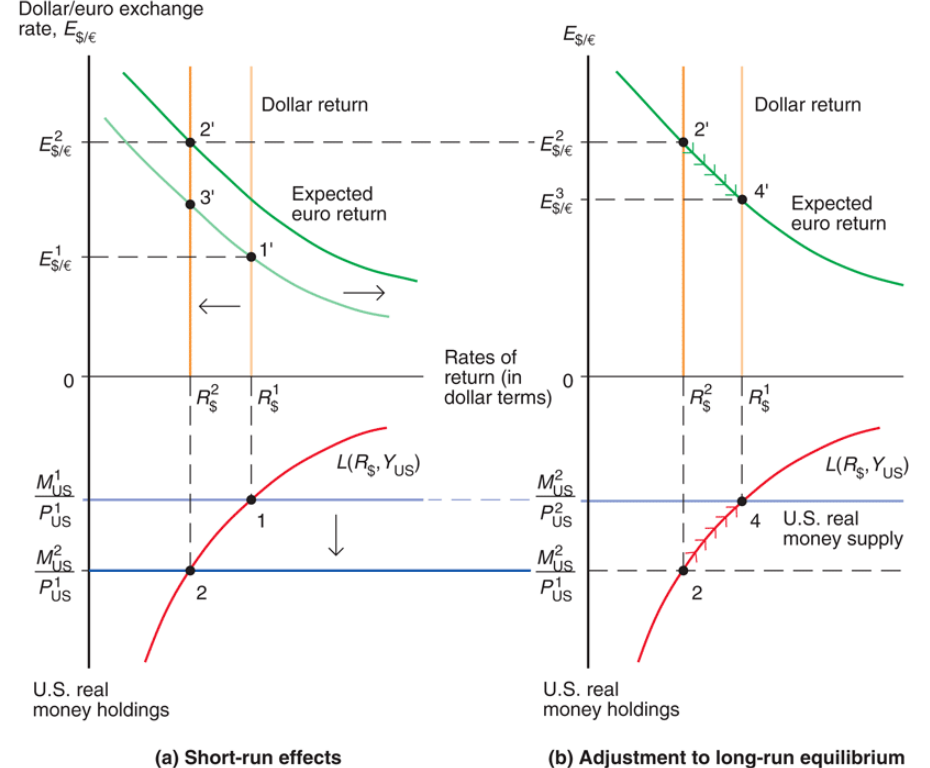
\includegraphics[scale=0.25]{long_run_exchange.png}
\end{figure}
}

\frame{
\frametitle{Long-run interest rate changes}
\begin{itemize}
    \item What could cause a permanent (long-run) change in the interest rate?
    \item Solution: a change in the growth rate of money supply (inflation)
\end{itemize}
}

\frame{
\frametitle{Inflation}
\begin{itemize}
\item Central banks in the real world typically gradually increases the money supply
\begin{itemize}
    \item Money supply grows at a constant rate
    \item Price inflation at the same rate
\end{itemize}
\end{itemize}
}

\frame[plain]{
\frametitle{Inflation and interest rates}
\begin{itemize}
    \item Interest rate parity still has to hold:
\begin{center}
$R_{USD,t}= R_{EURO,t}+\left(\frac{E^{e}_{USD/EURO,t+1}-E_{USD/EURO,t}}{E_{USD/EURO,t}}\right)$
\end{center}
    \item Relative PPP holds (implied by absolute PPP)
\begin{center}
$\frac{\left(E_{USD/EURO,t} - E_{USD/EURO,t-1}\right)}{ E_{USD/EURO,t-1}}= \pi_{US, t} - \pi_{E, t}$
\end{center}
\begin{center}
$R_{USD} - R_{EURO} = \pi^{e}_{US} - \pi^{e}_{E}$
\end{center}
or
\begin{center}
$R_{USD} - \pi^{e}_{US} = R_{EURO}- \pi^{e}_{E}$
\end{center}
\item \emph{Real} interest rates are the same
\end{itemize}
}

\frame{
\frametitle{The Fisher Effect}
\begin{center}
$R_{USD} - R_{EURO} = \pi^{e}_{US} - \pi^{e}_{E}$
\end{center}
\begin{itemize}
\item A rise in a country's expected inflation rate will eventually cause an equal rise in the interest rate that deposits of its currency offer
\begin{itemize}
\item In the long run, purely monetary developments should have no real effects (neutrality of money)
\item Expected growth in money supply affects the interest rate through inflation
\end{itemize}
\end{itemize}
}

\frame{
\frametitle{Interest and Monetary Policy}
\begin{itemize}
\item If growth in $M^{s}_{US}$ changes permanently from $\pi$ to $\pi+\Delta\pi$ (and $M^{s}_{E}$ is constant) such that $\pi_{US, t}$ and $\pi^{e}_{US}$ increases from $\pi$ to $\pi+\Delta\pi$
\item $R_{US}$ increases by $\Delta\pi$ (and $R_{e}$ is unchanged)
\end{itemize}
}

\frame[plain]{
\frametitle{Money growth and exchange rates}
\begin{figure}
	\centering
		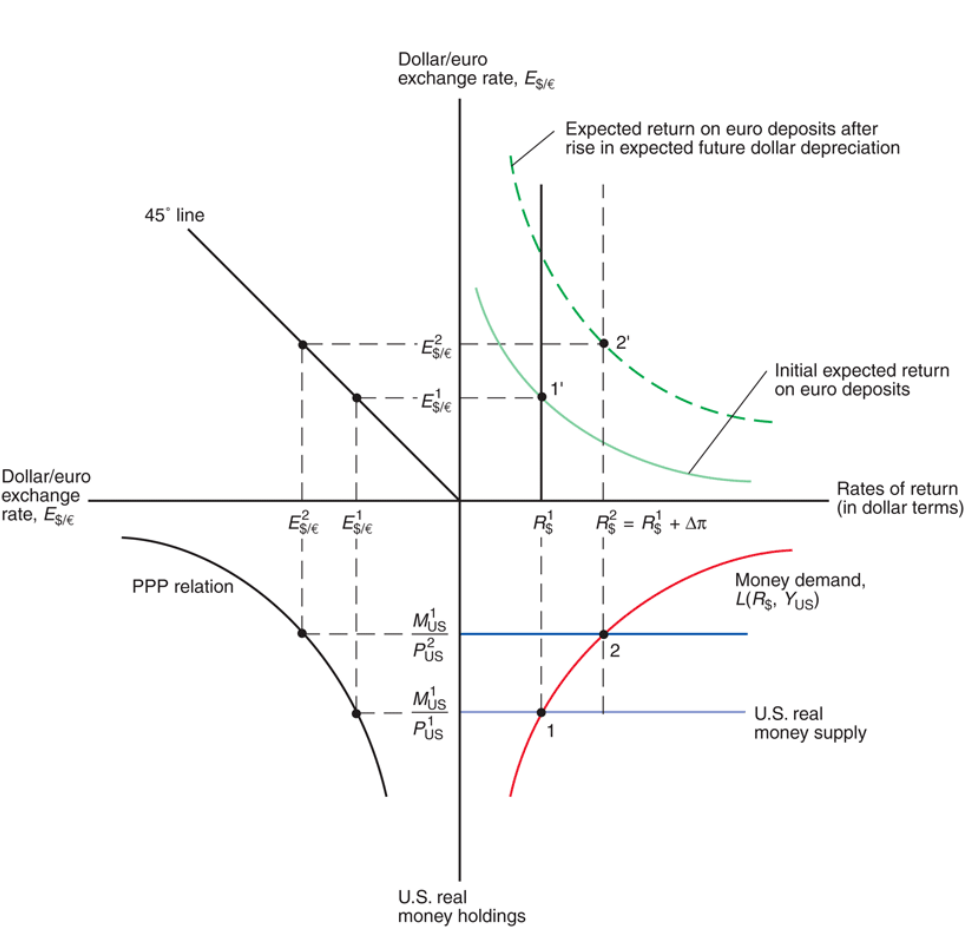
\includegraphics[scale=0.25]{money_growth_exchange.png}
\end{figure}
}

\frame[plain]{
\frametitle{(Long-term) Time trends following a change in growth rate}
\begin{figure}
	\centering
		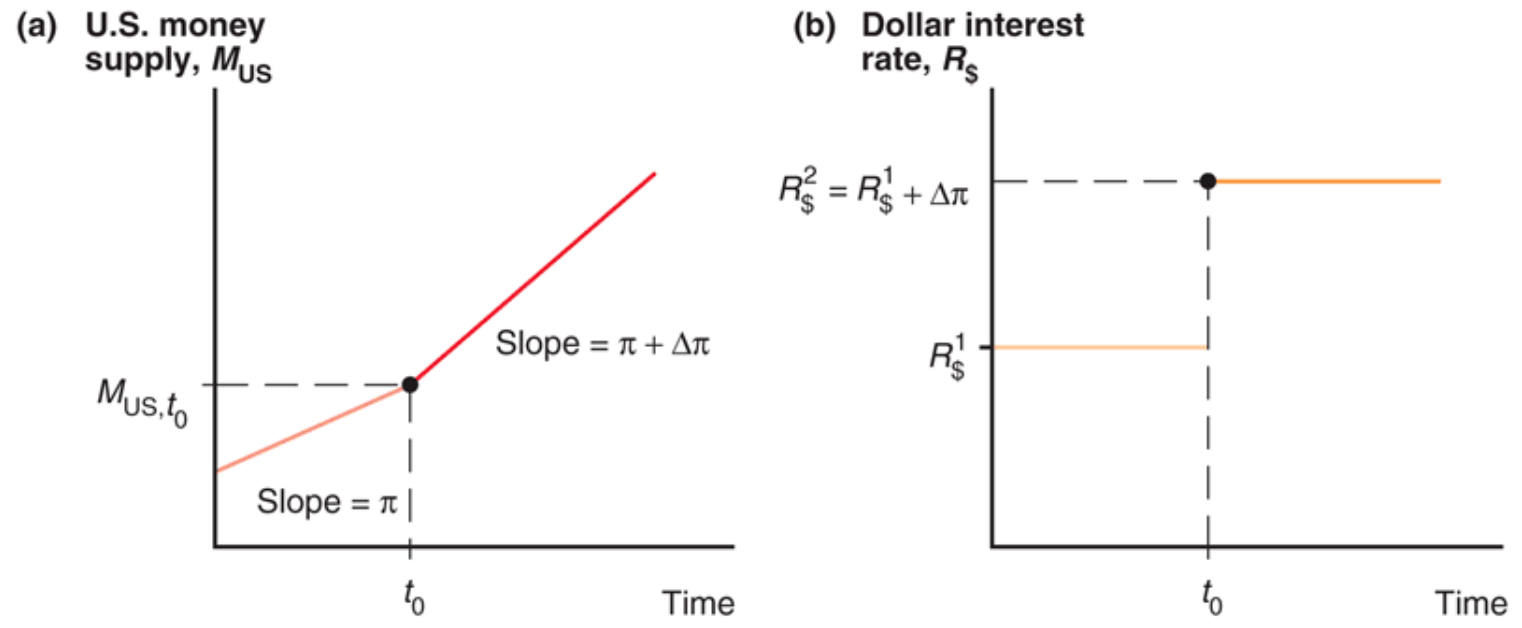
\includegraphics[scale=0.20]{time_trends1.png}
\end{figure}
}

\frame[plain]{
\frametitle{(Long-term) Time trends following a change in growth rate}
\begin{figure}
	\centering
		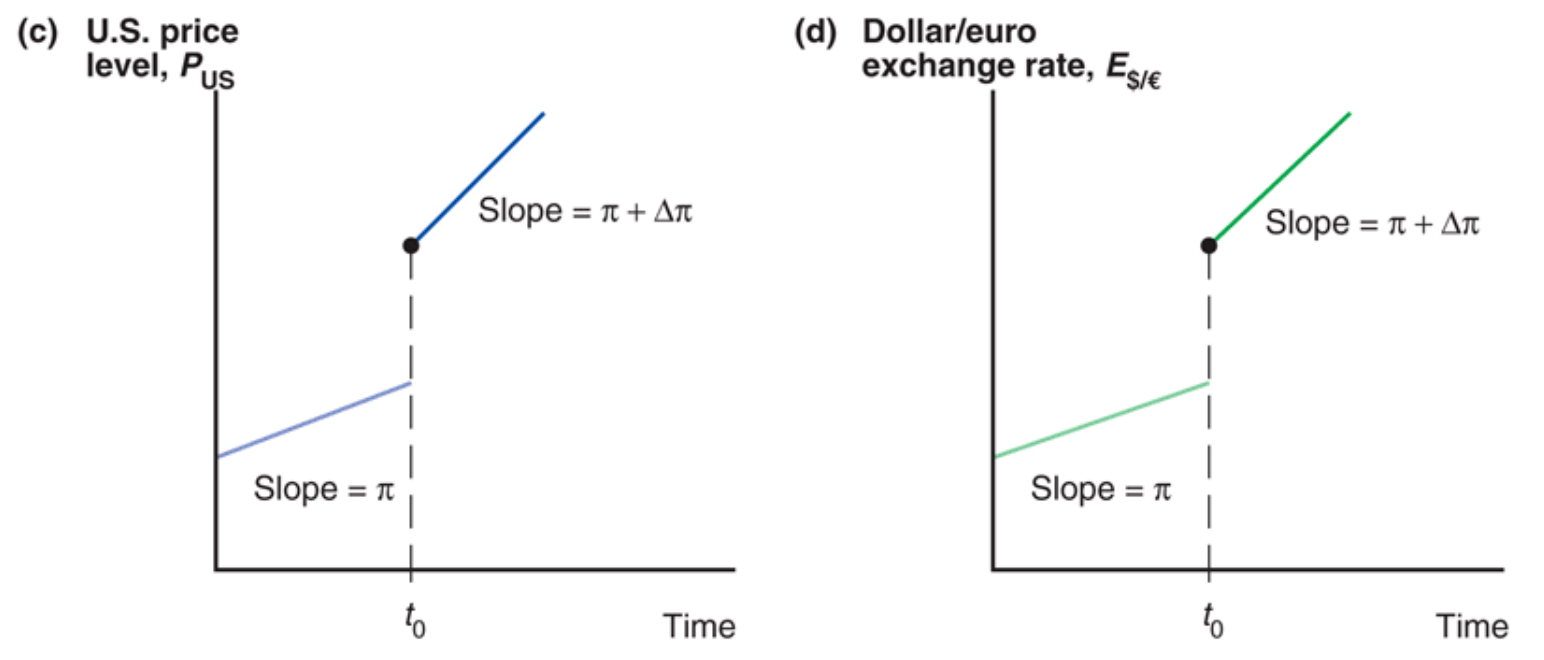
\includegraphics[scale=0.20]{timetrends2.png}
\end{figure}
}

\begin{frame}{Pause}

    \begin{itemize}
        \item We defined Purchasing Power Parity
        \item We derived the inflation rate/rate of return connection 
        \item We saw the three predictions of the PPP long-run model
        \begin{itemize}
            \item $M^{s}_{US}  \Uparrow \Rightarrow E_{\$/\text{\euro}}\Uparrow$  
            \item $R_{USD}  \Uparrow \Rightarrow E_{\$/\text{\euro}}\Uparrow$
            \item $Y_{US} \Uparrow \Rightarrow E_{\$/\text{\euro}}\Downarrow$ 
        \end{itemize}
        \item Next empirical evidence on the PPP long-run model
        \begin{itemize}
            \item Preview: Not good
        \end{itemize}
    \end{itemize}

\end{frame}

\frame{
\frametitle{Empirical Evidence on PPP (1)}
\begin{itemize}
\item The empirical support for PPP and
the law of one price is weak.
\item The prices of identical commodity
baskets, when converted to a single
currency, differ substantially across
countries.
\item Relative PPP also performs poorly.
\end{itemize}}


\frame[plain]{
\frametitle{The Yen/Dollar Exchange Rate and Relative Japan-U.S. Price Levels, 1980-2012}
\begin{figure}
	\centering
		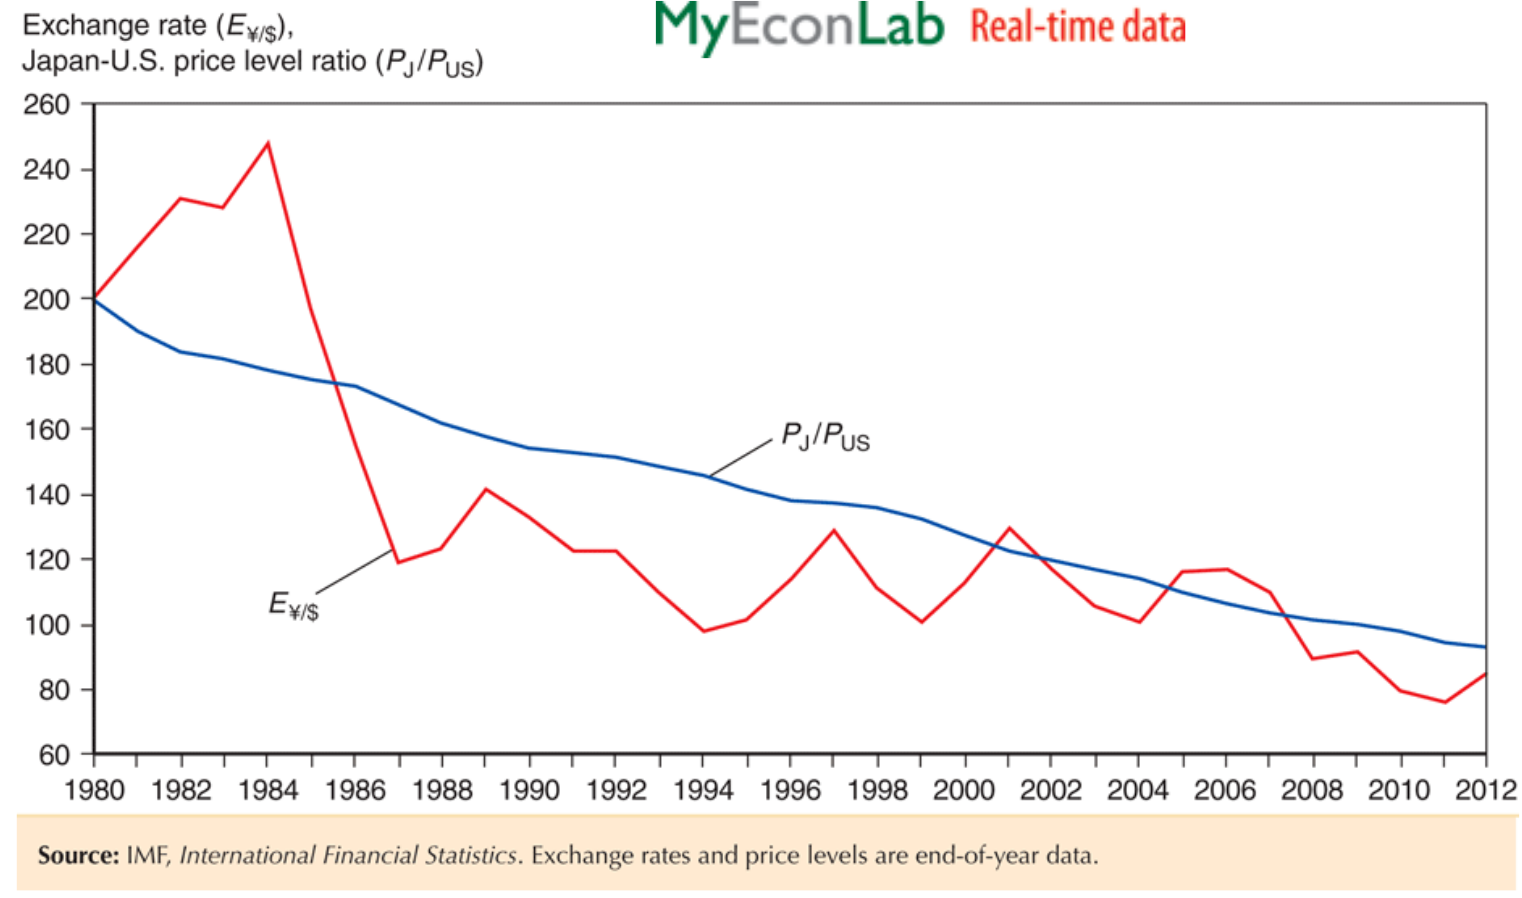
\includegraphics[scale=0.2]{yen_dollar.png}
	\label{fig:11}
\end{figure}
}


\frame[plain]{
\frametitle{Big Mac Index}
\begin{figure}
	\centering
		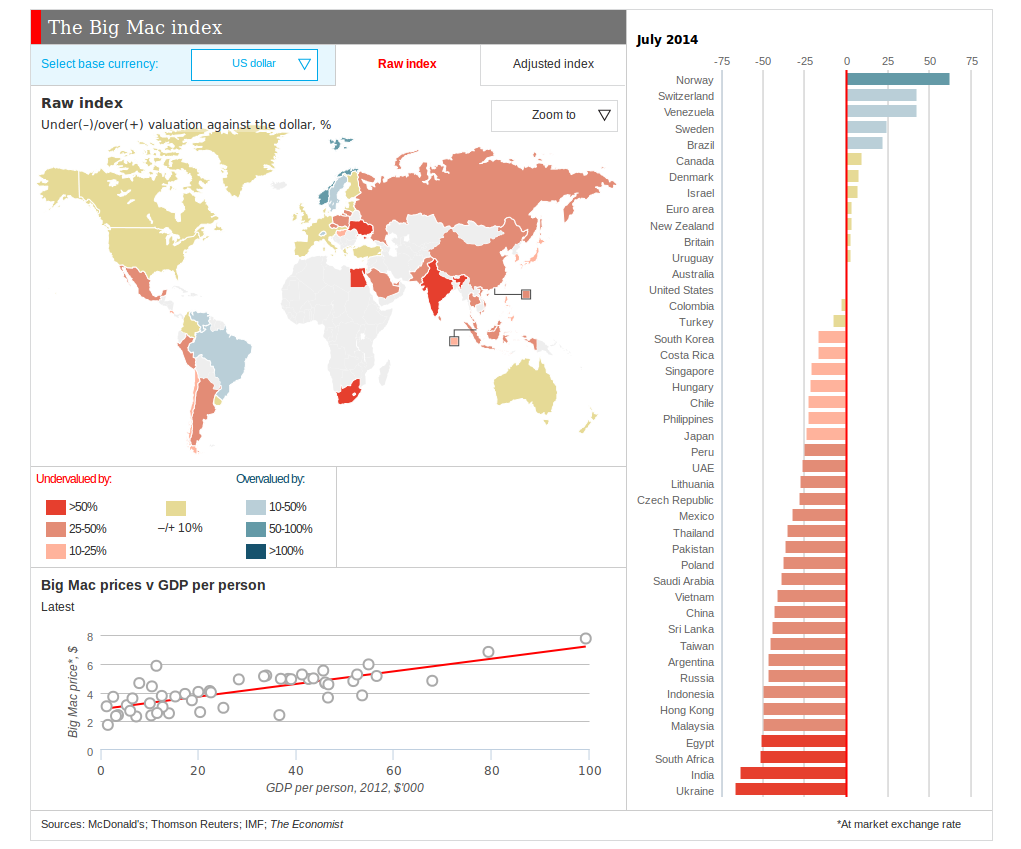
\includegraphics[scale=0.25]{big_mac_economist.png}
\end{figure}
}

\frame[plain]{
\frametitle{Big Mac Index - Denmark}
\begin{figure}
	\centering
		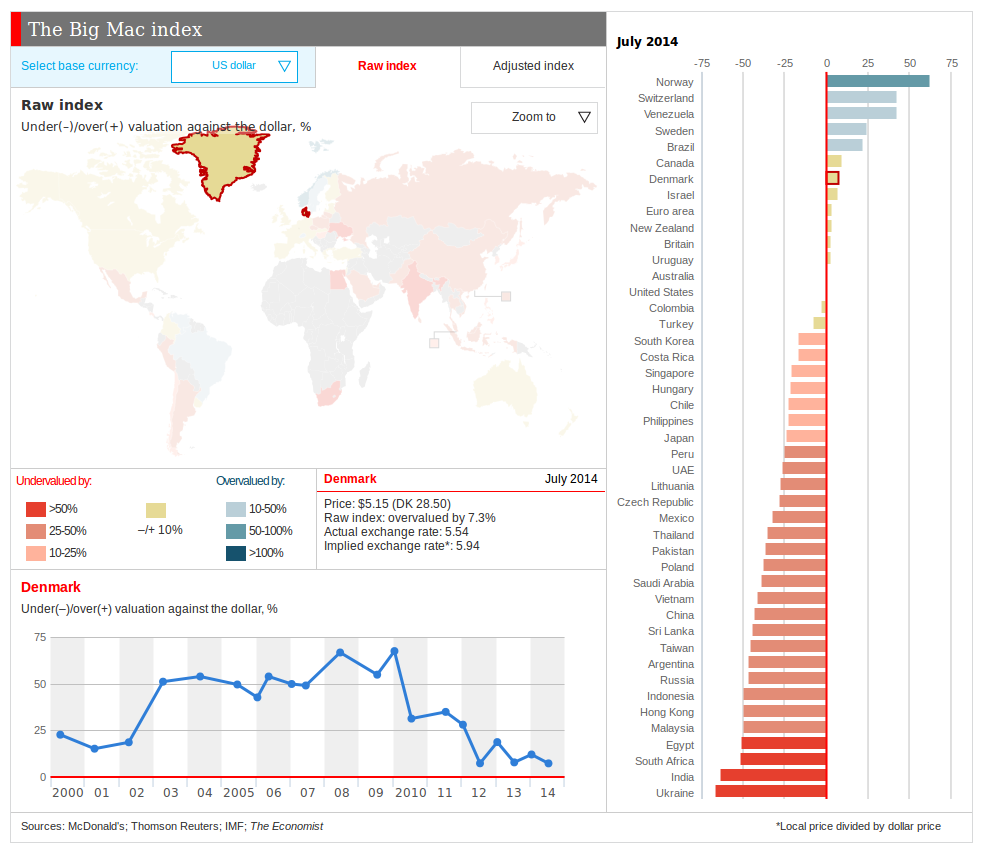
\includegraphics[scale=0.25]{big_mac_denmark.png}
\end{figure}
}

\frame[plain]{
\frametitle{Balassa Samuelson theory}
\begin{figure}
	\centering
		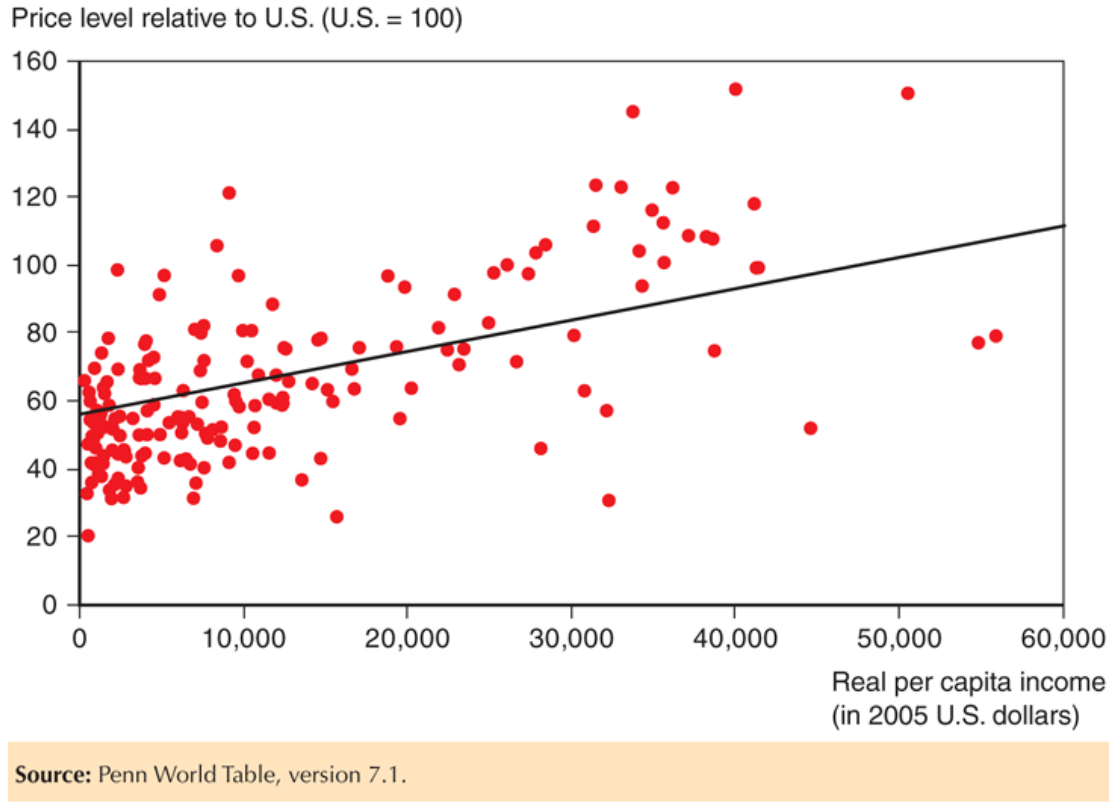
\includegraphics[scale=0.25]{balassa_samuelson.png}
\end{figure}
}

\frame{
\frametitle{Why does PPP do so badly}
\begin{enumerate}
\item Trade barriers and non-tradable products 
\item Imperfect competition
\item Differences in measures of average prices for baskets of goods and services
\end{enumerate}
}

\frame{
\frametitle{Trade barriers and non-tradables}
\begin{itemize}
\item Trade policy -- trade barriers drive a wedge between prices
\item Transport costs are a non-negligible trade barrier
\item Non-tradables enter consumption basket, cheaper in developing countries
\item This explains departure from absolute PPP, but not relative PPP!
\end{itemize}
}

\frame{
\frametitle{Pricing to market}
\begin{itemize}
    \item Companies that export charge each country a different price
    \item Strong evidence that this is happening
    \item Markups are complicated
\end{itemize}
}

\frame{
\frametitle{Basket differences}
\begin{itemize}
    \item Data on price levels based on government baskets
    \item Governments use baskets to make CPI 
    \item Baskets differ between countries
    \item Baskets also differ over time!
    \item Can screw up both relative and absolute PPP
\end{itemize}
}

\frame{
\frametitle{Swedish-Finish duty free}
\begin{itemize}
    \item Paper by Marcus Asplund, my colleague
    \item Sweden to Finland ferry duty free
    \begin{itemize}
        \item Duty free catelogue printed only occassionally
        \item Exchange rate fluctuations made PPP violations
        \item Still Swedes paid kroner, and Finns paid markka
        \item Even when printing, some pricing to market 
    \end{itemize}
    \item Empirical evidence that prices are sticky
    \item Empirical evidence of pricing to market
\end{itemize}
}


% \frame{
% \frametitle{A General Model of Long-Run
% Exchange Rates (1)}
% The Real Exchange Rate
% \begin{itemize}
% \item Measure of the prices of one country's
% goods and services relative to the other's.
% \item The real exchange rate is the dollar price of
% the European basket relative to that of the
% US price:
% \begin{center}
% $q_{USD/EURO} = \frac{\left(E_{USD/EURO} x P_{E}\right)}{P_{US}}$
% \end{center}
% \item Observe that PPP only holds for $q_{USD/EURO}=1$
% (absolute) or $q_{USD/EURO,t}-q_{USD/EURO,t-1}=0$ (conditional)
% \end{itemize}}
% 
% \frame{
% \frametitle{A General Model of Long-Run
% Exchange Rates (2)}
% \begin{enumerate}
% \item Real depreciation (q increases): If US
% prices fall in relation to foreign prices
% (measured in USD). This happens if:
% \begin{itemize}
% \item Nominal exchange rate depreciates (E
% increases), or
% \item US prices fall, or
% \item Euroland prices increase
% \end{itemize}
% \item Real appreciation (q falls): If US prices
% increases relative to foreign prices
% (measured in USD). This happens if:
% \begin{itemize}
% \item Nominal exchange rate appreciates (E falls),
% or
% \item US prices increase, or
% \item Euroland prices fall
% \end{itemize}
% \end{enumerate}
% }
% 
% 
% 
% \frame{
% \frametitle{A General Model of Long-Run
% Exchange Rates (3)}
% We can express the nominal exchange
% rate as:
% \begin{center}
% $E_{USD/EURO} = q_{USD/EURO} x (\frac{P_US}{P_E})$
% \end{center}
% \begin{center}
% $\Rightarrow$
% \end{center}
% \begin{center}
% $\frac{q^{e}_{USD/EURO}-q_{USD/EURO}}{q_{USD/EURO}}=\frac{E^{e}_{USD/EURO}-E_{USD/EURO}}{E_{USD/EURO}}-\left(\pi^{e}_{US}-\pi^{e}_{EURO}\right)$
% \end{center}
% Combining with the interest parity condition, the international interest gap is equal to:
% \begin{center}
% $\frac{q^{e}_{USD/EURO}-q_{USD/EURO}}{q_{USD/EURO}}=\frac{E^{e}_{USD/EURO}-E_{USD/EURO}}{E_{USD/EURO}}-\left(\pi^{e}_{US}-\pi^{e}_{EURO}\right)$
% \end{center}
% \begin{center}
% $R_{US}-R_{EURO}=\frac{q^{e}_{USD/EURO}-q_{USD/EURO}}{q_{USD/EURO}}-\left(\pi^{e}_{US}-\pi^{e}_{EURO}\right)$
% \end{center}
% }
% 
% 
% \frame[plain]{
% \frametitle{Fig. 16-4: Determination of the Long-Run Real Exchange Rate}
% \begin{figure}
% 	\centering
% 		\includegraphics[width=0.85\textwidth]{154.pdf}
% 	\label{fig:11}
% \end{figure}
% }
% 
% 
% \frame[plain]{
% \frametitle{}
% \begin{figure}
% 	\centering
% 		\includegraphics[width=0.85\textwidth]{155.pdf}
% 	\label{fig:11}
% \end{figure}
% }
% 
% \frame{
% \frametitle{Real Interest parity}
% \begin{center}
% $r^{e}_{US} -� r^{e}_{EU} = \frac{\left(q^{e}_{US/EU} -q_{US/EU}\right)}{q_{US/EU}}$
% \end{center}
% This equation is called real interest parity.
% It says that differences in real interest rates (in terms of goods and services that are earned or forgone when lending or borrowing) between countries are equal to the expected change in the value/price/cost of goods and services between countries.
% }
% 
% \begin{frame}{Overall trade review}
% 
% \begin{tikzpicture}
% \tikzset{scale=0.75,grow'=right,level distance=70pt}
% \tikzset{execute at begin node=\strut}
% \tikzset{every tree node/.style={anchor=base west}}
% 
% \Tree   [.Int\ Econ                     [.Trade     [.Theory    [.Comparative\ advantage ]
%                                                                 [.Factor\ endowments ]
%                                                                 [.Specific\ factors ]
%                                                                 [.Scale\ economies ]
%                                                                 [.Standard\ model ] ]
%                                                     [.Policy    [.Policy\ instruments ]
%                                                                 [.Political\ economy ] ] ]
%                                         [.Finance   [.Theory    [.Terminology\ and\ principles ]
%                                                                 [.Long-run\ exchange\ rates ] ]
%                                                     [.Policy    [.Short-run\ exchange\ rates ]
%                                                                 [.Coordination\ and\ Currency\ unions ] ] ] ]
% \end{tikzpicture}
% \end{frame}





\end{document}
